%% bare_conf.tex
%% V1.3
%% 2007/01/11
%% by Michael Shell
%% See:
%% http://www.michaelshell.org/
%% for current contact information.
%%
%% This is a skeleton file demonstrating the use of IEEEtran.cls
%% (requires IEEEtran.cls version 1.7 or later) with an IEEE conference paper.
%%
%% Support sites:
%% http://www.michaelshell.org/tex/ieeetran/
%% http://www.ctan.org/tex-archive/macros/latex/contrib/IEEEtran/
%% and
%% http://www.ieee.org/

%%*************************************************************************
%% Legal Notice:
%% This code is offered as-is without any warranty either expressed or
%% implied; without even the implied warranty of MERCHANTABILITY or
%% FITNESS FOR A PARTICULAR PURPOSE! 
%% User assumes all risk.
%% In no event shall IEEE or any contributor to this code be liable for
%% any damages or losses, including, but not limited to, incidental,
%% consequential, or any other damages, resulting from the use or misuse
%% of any information contained here.
%%
%% All comments are the opinions of their respective authors and are not
%% necessarily endorsed by the IEEE.
%%
%% This work is distributed under the LaTeX Project Public License (LPPL)
%% ( http://www.latex-project.org/ ) version 1.3, and may be freely used,
%% distributed and modified. A copy of the LPPL, version 1.3, is included
%% in the base LaTeX documentation of all distributions of LaTeX released
%% 2003/12/01 or later.
%% Retain all contribution notices and credits.
%% ** Modified files should be clearly indicated as such, including  **
%% ** renaming them and changing author support contact information. **
%%
%% File list of work: IEEEtran.cls, IEEEtran_HOWTO.pdf, bare_adv.tex,
%%                    bare_conf.tex, bare_jrnl.tex, bare_jrnl_compsoc.tex
%%*************************************************************************

% *** Authors should verify (and, if needed, correct) their LaTeX system  ***
% *** with the testflow diagnostic prior to trusting their LaTeX platform ***
% *** with production work. IEEE's font choices can trigger bugs that do  ***
% *** not appear when using other class files.                            ***
% The testflow support page is at:
% http://www.michaelshell.org/tex/testflow/



% Note that the a4paper option is mainly intended so that authors in
% countries using A4 can easily print to A4 and see how their papers will
% look in print - the typesetting of the document will not typically be
% affected with changes in paper size (but the bottom and side margins will).
% Use the testflow package mentioned above to verify correct handling of
% both paper sizes by the user's LaTeX system.
%
% Also note that the "draftcls" or "draftclsnofoot", not "draft", option
% should be used if it is desired that the figures are to be displayed in
% draft mode.
%
\documentclass[10pt,conference,compsocconf]{IEEEtran}
%\documentclass[10pt]{IEEEtran}
\usepackage{times}
\usepackage{color}
\usepackage{caption}
\usepackage{graphicx}




\captionsetup{font=footnotesize,justification=centering,labelsep=period}

% Add the compsoc option for Computer Society conferences.
%
% If IEEEtran.cls has not been installed into the LaTeX system files,
% manually specify the path to it like:
% \documentclass[conference]{../sty/IEEEtran}





% Some very useful LaTeX packages include:
% (uncomment the ones you want to load)


% *** MISC UTILITY PACKAGES ***
%
%\usepackage{ifpdf}
% Heiko Oberdiek's ifpdf.sty is very useful if you need conditional
% compilation based on whether the output is pdf or dvi.
% usage:
% \ifpdf
%   % pdf code
% \else
%   % dvi code
% \fi
% The latest version of ifpdf.sty can be obtained from:
% http://www.ctan.org/tex-archive/macros/latex/contrib/oberdiek/
% Also, note that IEEEtran.cls V1.7 and later provides a builtin
% \ifCLASSINFOpdf conditional that works the same way.
% When switching from latex to pdflatex and vice-versa, the compiler may
% have to be run twice to clear warning/error messages.






% *** CITATION PACKAGES ***
%
%\usepackage{cite}
% cite.sty was written by Donald Arseneau
% V1.6 and later of IEEEtran pre-defines the format of the cite.sty package
% \cite{} output to follow that of IEEE. Loading the cite package will
% result in citation numbers being automatically sorted and properly
% "compressed/ranged". e.g., [1], [9], [2], [7], [5], [6] without using
% cite.sty will become [1], [2], [5]--[7], [9] using cite.sty. cite.sty's
% \cite will automatically add leading space, if needed. Use cite.sty's
% noadjust option (cite.sty V3.8 and later) if you want to turn this off.
% cite.sty is already installed on most LaTeX systems. Be sure and use
% version 4.0 (2003-05-27) and later if using hyperref.sty. cite.sty does
% not currently provide for hyperlinked citations.
% The latest version can be obtained at:
% http://www.ctan.org/tex-archive/macros/latex/contrib/cite/
% The documentation is contained in the cite.sty file itself.






% *** GRAPHICS RELATED PACKAGES ***
%
\ifCLASSINFOpdf
  % \usepackage[pdftex]{graphicx}
  % declare the path(s) where your graphic files are
  % \graphicspath{{../pdf/}{../jpeg/}}
  % and their extensions so you won't have to specify these with
  % every instance of \includegraphics
  % \DeclareGraphicsExtensions{.pdf,.jpeg,.png}
\else
  % or other class option (dvipsone, dvipdf, if not using dvips). graphicx
  % will default to the driver specified in the system graphics.cfg if no
  % driver is specified.
  % \usepackage[dvips]{graphicx}
  % declare the path(s) where your graphic files are
  % \graphicspath{{../eps/}}
  % and their extensions so you won't have to specify these with
  % every instance of \includegraphics
  % \DeclareGraphicsExtensions{.eps}
\fi
% graphicx was written by David Carlisle and Sebastian Rahtz. It is
% required if you want graphics, photos, etc. graphicx.sty is already
% installed on most LaTeX systems. The latest version and documentation can
% be obtained at: 
% http://www.ctan.org/tex-archive/macros/latex/required/graphics/
% Another good source of documentation is "Using Imported Graphics in
% LaTeX2e" by Keith Reckdahl which can be found as epslatex.ps or
% epslatex.pdf at: http://www.ctan.org/tex-archive/info/
%
% latex, and pdflatex in dvi mode, support graphics in encapsulated
% postscript (.eps) format. pdflatex in pdf mode supports graphics
% in .pdf, .jpeg, .png and .mps (metapost) formats. Users should ensure
% that all non-photo figures use a vector format (.eps, .pdf, .mps) and
% not a bitmapped formats (.jpeg, .png). IEEE frowns on bitmapped formats
% which can result in "jaggedy"/blurry rendering of lines and letters as
% well as large increases in file sizes.
%
% You can find documentation about the pdfTeX application at:
% http://www.tug.org/applications/pdftex





% *** MATH PACKAGES ***
%
%\usepackage[cmex10]{amsmath}
% A popular package from the American Mathematical Society that provides
% many useful and powerful commands for dealing with mathematics. If using
% it, be sure to load this package with the cmex10 option to ensure that
% only type 1 fonts will utilized at all point sizes. Without this option,
% it is possible that some math symbols, particularly those within
% footnotes, will be rendered in bitmap form which will result in a
% document that can not be IEEE Xplore compliant!
%
% Also, note that the amsmath package sets \interdisplaylinepenalty to 10000
% thus preventing page breaks from occurring within multiline equations. Use:
%\interdisplaylinepenalty=2500
% after loading amsmath to restore such page breaks as IEEEtran.cls normally
% does. amsmath.sty is already installed on most LaTeX systems. The latest
% version and documentation can be obtained at:
% http://www.ctan.org/tex-archive/macros/latex/required/amslatex/math/





% *** SPECIALIZED LIST PACKAGES ***
%
%\usepackage{algorithmic}
% algorithmic.sty was written by Peter Williams and Rogerio Brito.
% This package provides an algorithmic environment fo describing algorithms.
% You can use the algorithmic environment in-text or within a figure
% environment to provide for a floating algorithm. Do NOT use the algorithm
% floating environment provided by algorithm.sty (by the same authors) or
% algorithm2e.sty (by Christophe Fiorio) as IEEE does not use dedicated
% algorithm float types and packages that provide these will not provide
% correct IEEE style captions. The latest version and documentation of
% algorithmic.sty can be obtained at:
% http://www.ctan.org/tex-archive/macros/latex/contrib/algorithms/
% There is also a support site at:
% http://algorithms.berlios.de/index.html
% Also of interest may be the (relatively newer and more customizable)
% algorithmicx.sty package by Szasz Janos:
% http://www.ctan.org/tex-archive/macros/latex/contrib/algorithmicx/




% *** ALIGNMENT PACKAGES ***
%
%\usepackage{array}
% Frank Mittelbach's and David Carlisle's array.sty patches and improves
% the standard LaTeX2e array and tabular environments to provide better
% appearance and additional user controls. As the default LaTeX2e table
% generation code is lacking to the point of almost being broken with
% respect to the quality of the end results, all users are strongly
% advised to use an enhanced (at the very least that provided by array.sty)
% set of table tools. array.sty is already installed on most systems. The
% latest version and documentation can be obtained at:
% http://www.ctan.org/tex-archive/macros/latex/required/tools/


%\usepackage{mdwmath}
%\usepackage{mdwtab}
% Also highly recommended is Mark Wooding's extremely powerful MDW tools,
% especially mdwmath.sty and mdwtab.sty which are used to format equations
% and tables, respectively. The MDWtools set is already installed on most
% LaTeX systems. The lastest version and documentation is available at:
% http://www.ctan.org/tex-archive/macros/latex/contrib/mdwtools/


% IEEEtran contains the IEEEeqnarray family of commands that can be used to
% generate multiline equations as well as matrices, tables, etc., of high
% quality.


%\usepackage{eqparbox}
% Also of notable interest is Scott Pakin's eqparbox package for creating
% (automatically sized) equal width boxes - aka "natural width parboxes".
% Available at:
% http://www.ctan.org/tex-archive/macros/latex/contrib/eqparbox/





% *** SUBFIGURE PACKAGES ***
%\usepackage[tight,footnotesize]{subfigure}
% subfigure.sty was written by Steven Douglas Cochran. This package makes it
% easy to put subfigures in your figures. e.g., "Figure 1a and 1b". For IEEE
% work, it is a good idea to load it with the tight package option to reduce
% the amount of white space around the subfigures. subfigure.sty is already
% installed on most LaTeX systems. The latest version and documentation can
% be obtained at:
% http://www.ctan.org/tex-archive/obsolete/macros/latex/contrib/subfigure/
% subfigure.sty has been superceeded by subfig.sty.



%\usepackage[caption=false]{caption}
%\usepackage[font=footnotesize]{subfig}
% subfig.sty, also written by Steven Douglas Cochran, is the modern
% replacement for subfigure.sty. However, subfig.sty requires and
% automatically loads Axel Sommerfeldt's caption.sty which will override
% IEEEtran.cls handling of captions and this will result in nonIEEE style
% figure/table captions. To prevent this problem, be sure and preload
% caption.sty with its "caption=false" package option. This is will preserve
% IEEEtran.cls handing of captions. Version 1.3 (2005/06/28) and later 
% (recommended due to many improvements over 1.2) of subfig.sty supports
% the caption=false option directly:
%\usepackage[caption=false,font=footnotesize]{subfig}
%
% The latest version and documentation can be obtained at:
% http://www.ctan.org/tex-archive/macros/latex/contrib/subfig/
% The latest version and documentation of caption.sty can be obtained at:
% http://www.ctan.org/tex-archive/macros/latex/contrib/caption/




% *** FLOAT PACKAGES ***
%
%\usepackage{fixltx2e}
% fixltx2e, the successor to the earlier fix2col.sty, was written by
% Frank Mittelbach and David Carlisle. This package corrects a few problems
% in the LaTeX2e kernel, the most notable of which is that in current
% LaTeX2e releases, the ordering of single and double column floats is not
% guaranteed to be preserved. Thus, an unpatched LaTeX2e can allow a
% single column figure to be placed prior to an earlier double column
% figure. The latest version and documentation can be found at:
% http://www.ctan.org/tex-archive/macros/latex/base/



%\usepackage{stfloats}
% stfloats.sty was written by Sigitas Tolusis. This package gives LaTeX2e
% the ability to do double column floats at the bottom of the page as well
% as the top. (e.g., "\begin{figure*}[!b]" is not normally possible in
% LaTeX2e). It also provides a command:
%\fnbelowfloat
% to enable the placement of footnotes below bottom floats (the standard
% LaTeX2e kernel puts them above bottom floats). This is an invasive package
% which rewrites many portions of the LaTeX2e float routines. It may not work
% with other packages that modify the LaTeX2e float routines. The latest
% version and documentation can be obtained at:
% http://www.ctan.org/tex-archive/macros/latex/contrib/sttools/
% Documentation is contained in the stfloats.sty comments as well as in the
% presfull.pdf file. Do not use the stfloats baselinefloat ability as IEEE
% does not allow \baselineskip to stretch. Authors submitting work to the
% IEEE should note that IEEE rarely uses double column equations and
% that authors should try to avoid such use. Do not be tempted to use the
% cuted.sty or midfloat.sty packages (also by Sigitas Tolusis) as IEEE does
% not format its papers in such ways.





% *** PDF, URL AND HYPERLINK PACKAGES ***
%
%\usepackage{url}
% url.sty was written by Donald Arseneau. It provides better support for
% handling and breaking URLs. url.sty is already installed on most LaTeX
% systems. The latest version can be obtained at:
% http://www.ctan.org/tex-archive/macros/latex/contrib/misc/
% Read the url.sty source comments for usage information. Basically,
% \url{my_url_here}.





% *** Do not adjust lengths that control margins, column widths, etc. ***
% *** Do not use packages that alter fonts (such as pslatex).         ***
% There should be no need to do such things with IEEEtran.cls V1.6 and later.
% (Unless specifically asked to do so by the journal or conference you plan
% to submit to, of course. )


% correct bad hyphenation here
\hyphenation{op-tical net-works semi-conduc-tor}

%\parskip 6pt plus 2pt minus 1pt
\parskip 3pt plus 2pt minus 1pt

\pagestyle{empty}
\begin{document}
\pagenumbering{gobble}
%
% paper title
% can use linebreaks \\ within to get better formatting as desired
\title{\textbf{\Large Computer Vision-based System for Impaired Human Vision Compensation}} % \\[-1.5ex] and subtitle}\\[0.2ex]}

% author names and affiliations
% use a multiple column layout for up to three different
% affiliations
\author{\IEEEauthorblockN{~\\[-0.4ex]\large Povilas Daniu\v{s}is\\[0.3ex]\normalsize}
\IEEEauthorblockA{Vilnius Gediminas Technical University\\
Vilnius, Lithuania}
\and
\IEEEauthorblockN{~\\[-0.4ex]\large Audrius Indriulionis\\[0.3ex]\normalsize}
\IEEEauthorblockA{Vilnius Gediminas Technical University\\
Vilnius, Lithuania}
\and
\IEEEauthorblockN{~\\[-0.4ex]\large Andrius Budrionis\\[0.3ex]\normalsize}
\IEEEauthorblockA{Vilnius Gediminas Technical University\\
Vilnius, Lithuania\\
Norwegian Centre for E-health Research\\
University Hospital of North Norway\\
Tromsø, Norway}}

% conference papers do not typically use \thanks and this command
% is locked out in conference mode. If really needed, such as for
% the acknowledgment of grants, issue a \IEEEoverridecommandlockouts
% after \documentclass

% for over three affiliations, or if they all won't fit within the width
% of the page, use this alternative format:
% 
%\author{\IEEEauthorblockN{Michael Shell\IEEEauthorrefmark{1},
%Homer Simpson\IEEEauthorrefmark{2},
%James Kirk\IEEEauthorrefmark{3}, 
%Montgomery Scott\IEEEauthorrefmark{3} and
%Eldon Tyrell\IEEEauthorrefmark{4}}
%\IEEEauthorblockA{\IEEEauthorrefmark{1}School of Electrical and Computer Engineering\\
%Georgia Institute of Technology,
%Atlanta, Georgia 30332--0250\\ Email: see http://www.michaelshell.org/contact.html}
%\IEEEauthorblockA{\IEEEauthorrefmark{2}Twentieth Century Fox, Springfield, USA\\
%Email: homer@thesimpsons.com}
%\IEEEauthorblockA{\IEEEauthorrefmark{3}Starfleet Academy, San Francisco, California 96678-2391\\
%Telephone: (800) 555--1212, Fax: (888) 555--1212}
%\IEEEauthorblockA{\IEEEauthorrefmark{4}Tyrell Inc., 123 Replicant Street, Los Angeles, California 90210--4321}}




% use for special paper notices
%\IEEEspecialpapernotice{(Invited Paper)}




% make the title area
\maketitle


\begin{abstract}
%\boldmath
In this short article we describe and discuss architecture of computer vision-based system for partial compensation of lost or impaired human vision.
\end{abstract}
% IEEEtran.cls defaults to using nonbold math in the Abstract.
% This preserves the distinction between vectors and scalars. However,
% if the conference you are submitting to favors bold math in the abstract,
% then you can use LaTeX's standard command \boldmath at the very start
% of the abstract to achieve this. Many IEEE journals/conferences frown on
% math in the abstract anyway.

% no keywords

\begin{IEEEkeywords}
Computer vision; Mobile application; Aid for blind and visually impaired; Tactile feedback; Impaired human vision compensation.%
\end{IEEEkeywords}



% For peer review papers, you can put extra information on the cover
% page as needed:
% \ifCLASSOPTIONpeerreview
% \begin{center} \bfseries EDICS Category: 3-BBND \end{center}
% \fi
%
% For peerreview papers, this IEEEtran command inserts a page break and
% creates the second title. It will be ignored for other modes.
\IEEEpeerreviewmaketitle


\section{Introduction}
\label{sec:introduction}

More than $250$ million people worldwide have moderate to severe vision impairment, while ($\approx 36$ million are blind) \cite{Bourne}. During the past decades significant effort was devoted to develop computer vision and other sensor based aids (e.g. \cite{Caraiman}, \cite{Csapo}, \cite{Poggi}, \cite{Zientara}) for helping the blind and visually impaired users to perceive the surrounding world. However, computer vision is rapidly evolving field, and systems based on the aforementioned approaches often lack accuracy and reliability in real-world conditions. In this article we describe a system, which employs modern computer vision techniques for compensation of lost or impaired vision function in humans. Many of the previously proposed electronic aids for the blind count on highly specialized hardware, for instance smart glasses \cite{Zientara}, Microsoft Kinnect sensors \cite{Owayjan}, helmet-mounted photo sensors and cameras \cite{Dunai}. Such systems often lack convenience and brings additional complexity into daily tasks, which visually impaired people currently manage by the help of a white cane. This project puts major emphasis on developing a tool, which seamlessly integrates with the hardware visually impaired person already has on-hand and is used to (smartphone). %This paper describes a high level architecture of the proposed technology aid for visually impaired people %(kartojasi su In this article we describe a system, which employs modern computer vision ...)


\section{Method}
\label{sec:method}

Following the principles of participatory design \cite{Kensing}, \cite{Carroll} we included the final users into the design process of the system. Two visually impaired persons participated in discussion and focus group meetings together with the project team to identify the key properties of the solution. During the six discussion sessions major attention was paid to:
\begin{enumerate}
\item Functionality and key features of the solution addressing real-life scenarios of visually impaired persons;
\item Technical feasibility, connecting user needs to the latest development in computer vision and assisted technologies;
\item Interface between the visually impaired person and the assisted technology;
\item Appearance, usability and potential costs of the final product. 
\end{enumerate}
Design process involved testing of the existing mobile phone app (Seeing AI) for assisting visually impaired persons. Semi-structured tests were performed by the visually impaired participants accompanied by a researcher from a project group. Strengths and weaknesses of the existing solutions are reflected in the design of the proposed system. 



\section{Results}
\label{sec:results}

User-centered design sessions with visually impaired persons provided substantial input for the design of the proposed system (Fig.~\ref{fig:schematics}). The process made it clear that understanding of the user needs was limited in the project group. Based on the results of the user-centered design process, we present the outline of the system for impaired human vision compensation. 

The key part of the proposed system is a smartphone device, connecting user interface and data processing components into a well-functioning ecosystem. Smartphone was selected due to its high availability and capability to perform required computations or forward visual information for processing to the external server via the Internet connection.

The cornerstones of the proposed solution are its inferface and external server, capable running computationally demanding modern image processing algorithms.

The interface consists of a wearable forehead belt, integrating RGB and depth cameras, tactile feedback device and bone conductive headphones. Altough more expensive than standard ones, bone conductive headphones allow the user to perceive audio information from the surrounding environment, which is essential for the visually impaired people.

External server processes received visual data according to user request with computer vision algorithms: faster RCNN object detector \cite{Ren}, trained to detect important objects, CNN-RNN-based scene description \cite{Liu}, place recognition \cite{Ohn-Bar}, face recognition \cite{Amos}, obstacle detection \cite{Laina}, among others. After completing an analysis this server transmits feedback signal back to the smartphone device for presenting it to the user via the above described interface.



%\begin{wrapfigure}{r}{0.4\textwidth}
\begin{figure}
  \begin{center}
    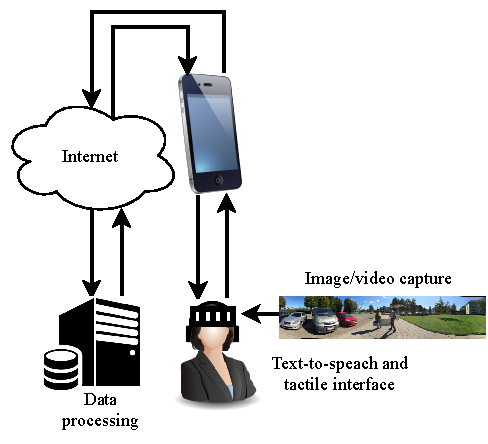
\includegraphics[scale=0.7]{./img/cropped_diagram.pdf}  
  \end{center}
  \caption{Schematics of vision compensation device.}
  \label{fig:schematics}
\end{figure}



%\end{wrapfigure}

%Following the above methodology we suggest the impaired human vision compensation system (\textbf{HVCS}), consisting of \textbf{Device} and \textbf{Inference} components (see Fig.~\ref{fig:schematics}).

%padalijimas i 2 komponentus man nelabai aiskus. As dalinciau i input (kameros, sensoriai), output (ausines, vibratoriu matricos), processing (local, remote). 
% tai kas dabar yra prie Inference, siulau perfrazuot kaip Functionality, ka as minejau Method. Taip pat visa Results skyreli reiktu labiau susiet su Method. Reiktu, kad visi 4 Method pamineti punktai isrysketu ir Results. 
%Results skyrelyje nereiktu taip stipriai fokusuotis i kitu grupiu tyrimus ir juos cituoti. Rezultatai juk musu.


Discussions on functionality and key features of the solution revealed a gap between the aims of the existing tools, which are often focused on advanced navigation and scene description features, and actual user needs. For example, the end users highlighted that a simplistic solution for navigating is lacking. 
%They were not excited about advanced object detection and scene description techniques, which may overcomplicate their daily life. 
Major focus was put on a easy to use and minimalistic tool, which can be trusted. Reliable object detection, direction and approximate distance to an obstacle were highlighted as major requirements. To our surprise, only 5-8 distinctive object classes (for instance, buss stop, pedestrian crossing, doors, stairs, etc) were of major importance while navigating. Additional information, such as type of a passing car, blossoming flowers in the park or person passing riding a bicycle was considered as overwhelming and distractive. 

%Social networking functionality was accepted as a potentially important feature allowing other users/volunteers to describe certain objects (for instance, temporary road works) with exact location and description. Navigating around such obstacles can be challenging for computer vision-based tools and may decrease user's trust in the tool. Integration of additional information from other users, governmental organizations and volunteers could be of high value for the visually impaired people. 

%Povilai, paziurek ar cia viskas OK, pridek ka nors nuo saves
Computer vision technology is under rapid development and during last years made major breakthrough in performance and efficiency. Deep learning neural networks, which are de facto standard in modern image/video processing, are now well supported by software libraries and dedicated hardware built-in even in relatively low-power computational devices, such as smartphones. These devices are also equipped with 4G Internet connectivity and sufficient computational power to perform initial data processing locally. The maturity of the aforementioned technologies suggest that our proposed computational aid for visually impaired persons may be highly feasible. 


The cornerstone of this project is the interface between the visually impaired person and the assistive technology. We are proposing a combination of audio and tactile feedback, which may improve the interaction between the assitive technology and the user. Similar interfaces were suggested by research communities earlier \cite{Zientara}, \cite{Poggi}, however, current knowledge on user preferences and evaluation of various options of tactile feedback (placement on the body, frequencies, strength, etc.) is limited. 

Appearance, usability and cost of the final solution is of major importance to the users. The proposed assistive technology should supplement the tool that visually impaired persons used for decades - the white cane. Using a white cane requires little to none training, has very low costs and is relatively reliable. It provides information on the surrounding objects 1-2 meters in front of the user. While the cane can used to detect a nearby obstacle, electronic travel aid could be beneficial for longer range (10-20m) route planning and object recognition. However, it should integrate seamlessly into the existing navigation practices of visually impaired people. 


 

%The proposed system  consists of three major parts: is a computational device the user currently uses for completing other daily tasks. It consists of sensors and actuators, integrated into smartphone-based computational core, which was chosen due its avialability to wide population, and capability to perform the required computations or forward visual information to the external server via the Internet connection. Sensors are mounted on forehead belt include: RGB camera, depth camera, IMU. Actuator set consists of bone conductive headphones, and head belt for presenting tactile-feedback to the user. %We suggest to use bone conductive headphones, ... 

%\textbf{Inference} subsystem consists of server computer with internet connection and set of computer vision algorithms, selected according to our methodology ed (see. Sec.~\ref{sec:method}): Faster RCNN object detector \cite{?}, trainto detect important objects (doors, floors, elevators, stairs, corridor junctions, etc.), CNN-RNN-based scene description \cite{Liu},\cite{Ren}, \cite{Dai}, place recognition \cite{Ohn-Bar}, face recognition \cite{Amos}, obstacle detection \cite{Laina}, and possibly other modules. 

%HVCS operation cycle is started by \textbf{Device} reading sensor data and transmitting it to the server for an analysis. Server calculates feedback signal and transmits it back to the device for presenting to the user.

\section{Discussion}
\label{sec:discussion}
%Didzioji Discussion teksto dalis man labiau tinka prie Results/Conclusion. Gal galim padiskutioti daugiau apie Limitations, Future Implications, Lessons Learned ar pan... Cia galime savo siuloma sistema lyginti su anksciau publikuotais rezultatais. 


In this article we outlined an idea of complex computer vision-based sensor architecture, which can help to partially compensate impaired or lost human sight. Main advantages of therein suggested system are: ability to use efficient (but still computationally intensive) modern computer vision algorithms via Internet connection, present the signal to the user by combined bone conductive headphone-tactile actuator, comparatively low cost and consequently increased potential availability of the device. The suggested system also integrates well with the main blind person's aid - the white cane. The hardware architecture can be used as the basis for various computer vision-based software modules, allowing to help visually impaired users in everyday routines (e.g. outdoor/indoor navigation, object/face recognition, obstacle detection, etc.). On the other side, due to remotelly conducted visual analysis, in some cases the suggested system may suffer from too large latency, its reliability depends on stability and quality of Internet connection. 



%The developed head-mounted tactile device is developed for head position and orientation tracking and could capture an image in front of visually impaired people. The tactile device with integrated 3D deph camera is integrated with smartphone by bluetooth which could preprocess the labeled image features. The developed high quality self navigation system is based on the computer vision methods especially enhancing the capabilities to detect and classify objects (e.g bus station, street crossings, ) with their surrounding objects. The authors expect to increase the capabilies of potentially blind to secure navigate especially for the planed destination (e.g. "home-office"). Work left (outdoor/indoor) etc.



% conference papers do not normally have an appendix


% use section* for acknowledgement
%\section*{Acknowledgment}
%The authors would like to thank...





% trigger a \newpage just before the given reference
% number - used to balance the columns on the last page
% adjust value as needed - may need to be readjusted if
% the document is modified later
%\IEEEtriggeratref{8}
% The "triggered" command can be changed if desired:
%\IEEEtriggercmd{\enlargethispage{-5in}}

% references section

% can use a bibliography generated by BibTeX as a .bbl file
% BibTeX documentation can be easily obtained at:
% http://www.ctan.org/tex-archive/biblio/bibtex/contrib/doc/
% The IEEEtran BibTeX style support page is at:
% http://www.michaelshell.org/tex/ieeetran/bibtex/
%\bibliographystyle{IEEEtran}
% argument is your BibTeX string definitions and bibliography database(s)
%\bibliography{IEEEabrv,../bib/paper}
%
% <OR> manually copy in the resultant .bbl file
% set second argument of \begin to the number of references
% (used to reserve space for the reference number labels box)
%
% As suggested below, edit bibtemplate_samples.bib to reflect
% your bibliography. See bibtemplate.text for referencing.
%

\bibliographystyle{IEEEtran}
%\bibliography{bibtemplate_samples}


\begin{thebibliography}{1}
\bibitem{Amos} Amos, B., Ludwiczuk, B., and Satyanarayanan, M. Openface:
A general-purpose face recognition library with mobile applications. Technical report, CMU-CS-16-118, CMU School of Computer Science, 2016.

\bibitem{Bourne} Bourne RRA, Flaxman SR, Braithwaite T, Cicinelli MV, Das A, Jonas JB, et al.; Vision Loss Expert Group. Magnitude, temporal trends, and projections of the global prevalence of blindness and distance and near vision impairment: a systematic review and meta-analysis. Lancet Glob Health.  2017 Sep;5(9):e888-97.

\bibitem{Caraiman} Caraiman, S., Morar, A., Owczarek, M.,Burlacu, A., Rzeszotarski, D., Botezatu, N., Herghelegiu, P., Moldoveanu, F., Strumillo, P., Moldoveanu, A. Computer Vision for the Visually Impaired: the Sound of Vision System. IEEE International Conference on Computer Vision Workshops, pp. 1480-1489, 2017.

\bibitem{Carroll} Carroll, J. M., Rosson, M. B. Participatory design in community informatics. Des. Stud., vol. 28, no. 3, pp. 243-261, May 2007.

\bibitem{Csapo} Csap\'{o}, A., Wers\'{e}nyi, G., Nagy, H., Stockman, T. A survey of assistive technologies and applications for blind users on mobile platforms: a review and foundation for research. Journal on Multimodal User Interfaces. Vol. 9, issule 4,  pp. 275-286, 2015.

\bibitem{Dunai} Dunai, L. D., Lengua, I. L., Tortajada, I., Brusola Simon, F. Obstacle detectors for visually impaired people. 2014 International Conference on Optimization of Electrical and Electronic Equipment (OPTIM), 2014. 

\bibitem{Kensing} Kensing, F., Simonsen, J., and B\o dker, K. MUST: A Method for Participatory Design. Hum-Comput Interact, vol. 13, no. 2, pp. 167-198, Jun. 1998.


\bibitem{Laina} Laina, I., Rupprecht, C., Belagiannis, V., Tombari, F., Navab, N. Deeper depth prediction with fully convolutional residual networks. Fourth International Conference on 3D Vision (3DV), pp. 239-248, 2016.

\bibitem{Liu} Liu, Ch., Mao, J., Sha, F., Yuille, A. Attention Correctness in Neural Image Captioning. Proceedings of the Thirty-First AAAI Conference on Artificial Intelligence, pp. 4176-4182, 2017.

\bibitem{Ohn-Bar}  Ohn-Bar, E., Kitani, K., Asakawa, Ch. Personalized Dynamics Models for Adaptive Assistive Navigation Interfaces. arXiv:1804.04118, [cs.LG], 2018.



\bibitem{Owayjan} Owayjan, M., Hayek, A., Nassrallah, H., Eldor, M. Smart Assistive Navigation System for Blind and Visually Impaired Individuals. 2015 International Conference on Advances in Biomedical Engineering (ICABME), 2015.

\bibitem{Poggi} Poggi, M., Mattoccia, S. A wearable mobility aid for the visually impaired based on embedded 3d vision and deep learning. Proceeding of IEEE Symposium on Compututers and Communication, pp. 208-213, 2016.

\bibitem{Ren} Ren, Sh., He, K., Girshick, R., and Sun, J.  Faster R-CNN: Towards real-time object detection with region proposal networks. In Advances in neural information processing systems, pp. 91-99, 2015.

\bibitem{Zientara} Zientara, P.,A., Lee, S., Smith, G., H., Brenner, R., Itti, L., Rosson M., B., Carroll, J., M., Irick K., M., Narayanan, V. Third Eye: A shopping assistant for the visually impaired. Computer Vol. 50, Issue 2, pp. 16-24, 2017.


%\bibitem{Poggi} Poggi, M., Mattoccia, S. A wearable mobility aid for the visually impaired based on embedded 3D vision and deep learning. 2016 IEEE Symposium on Computers and Communication (ISCC), 2016

\end{thebibliography}




% that's all folks
\end{document}


